\vspace{-1.5cm}
\begin{figure}[ht]
  \centering
  %
  \begin{subfigure}{0.31\linewidth}
  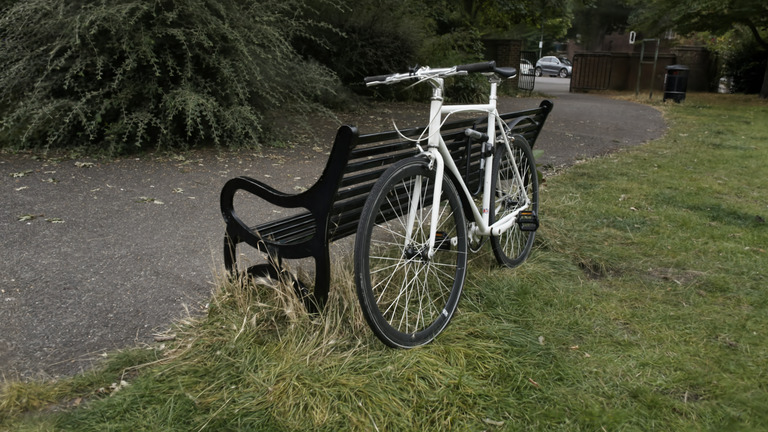
\includegraphics[width=\linewidth]{images/renders/bicycle_rgb_52.jpg}
  \end{subfigure}
  \hfill
  \begin{subfigure}{0.31\linewidth}
  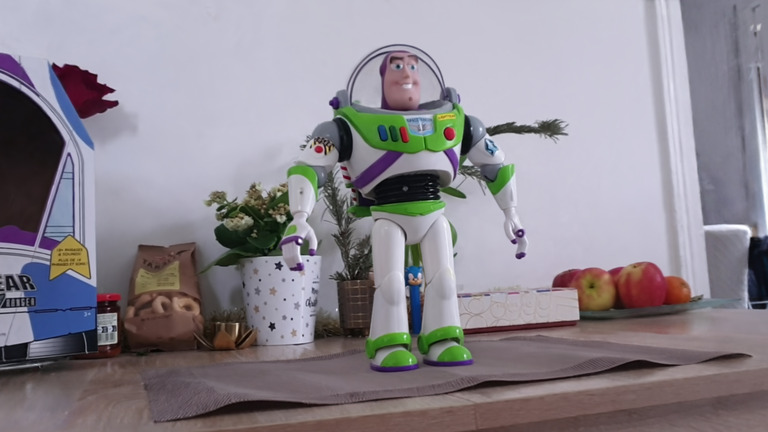
\includegraphics[width=\linewidth]{images/renders/buzz1_rgb_49.jpg}
  \end{subfigure}
  \hfill
  \begin{subfigure}{0.31\linewidth}
  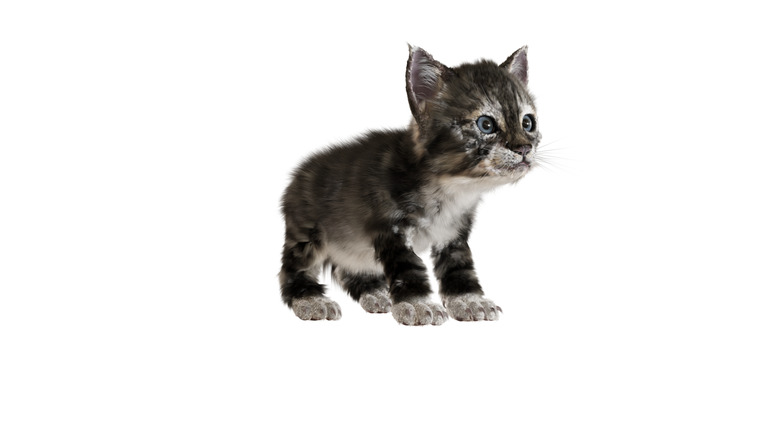
\includegraphics[width=\linewidth]{images/renders/kitten_rgb_42.jpg}
  \end{subfigure}\\
  {\small (a)~Rendering three different scenes with Frosting: \textit{Bicycle}, \textit{Buzz}, and \textit{Kitten}.}\\
  %
  \begin{subfigure}{0.49\linewidth}
  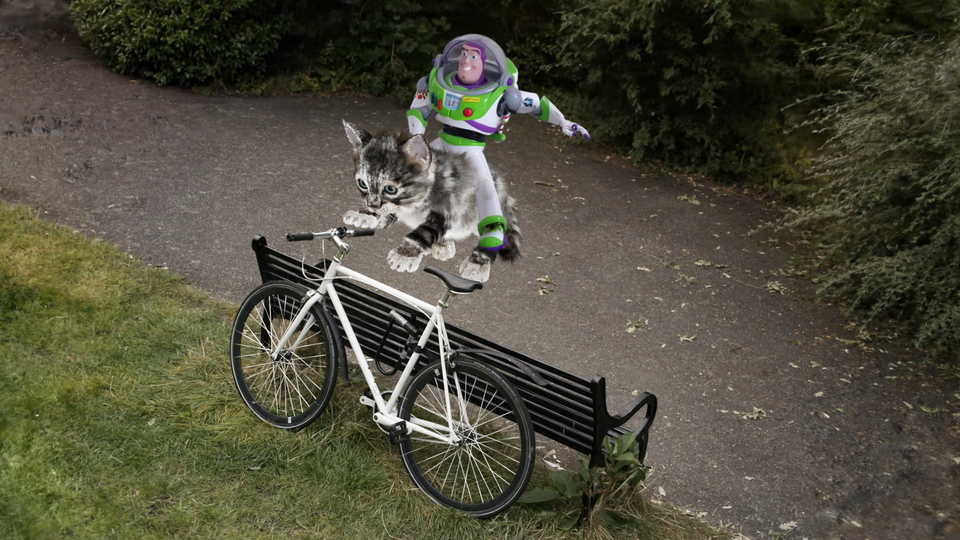
\includegraphics[width=\linewidth]{images/composition/buzz_riding_cat/0_0.png}
  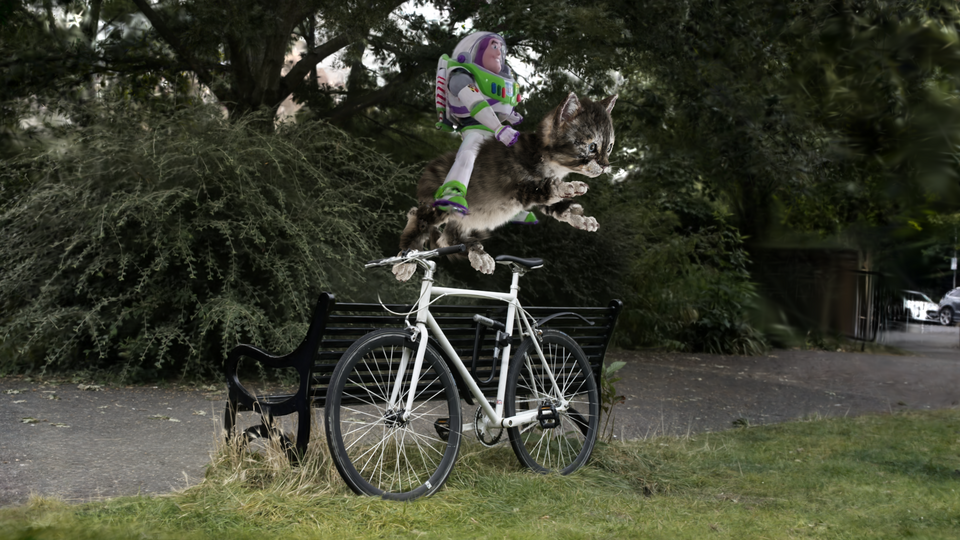
\includegraphics[width=\linewidth]{images/composition/buzz_riding_cat/0_3.png}
  \end{subfigure}
  \hfill
  \begin{subfigure}{0.49\linewidth}
  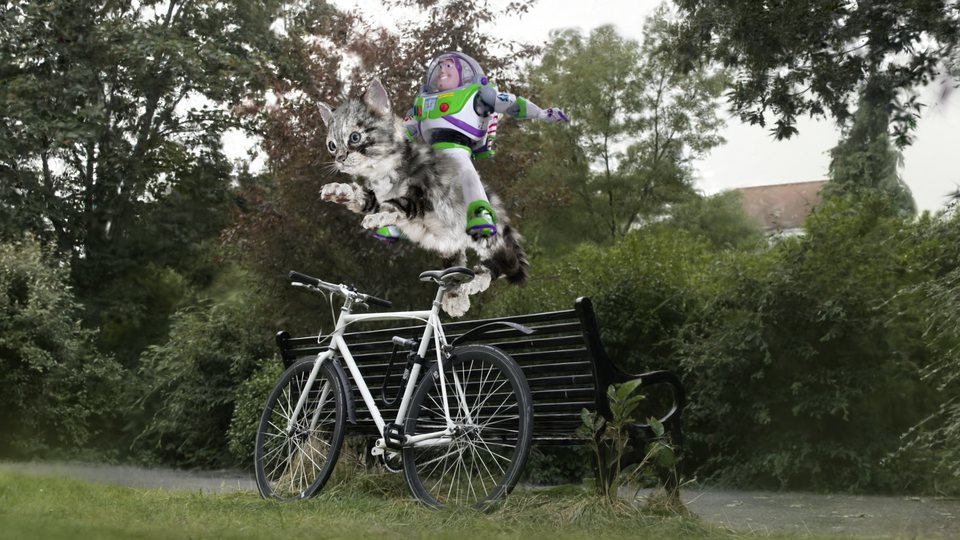
\includegraphics[width=\linewidth]{images/composition/buzz_riding_cat/0_1.png}
  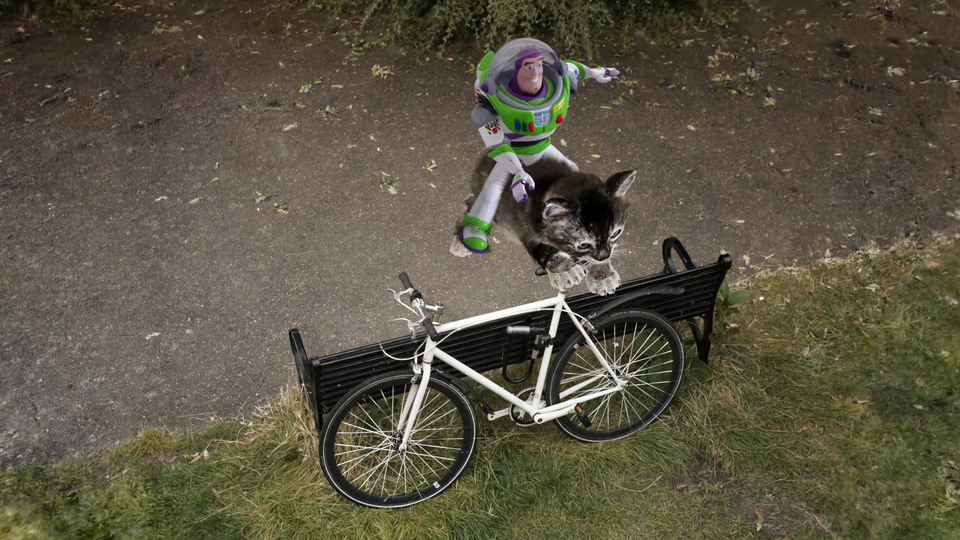
\includegraphics[width=\linewidth]{images/composition/buzz_riding_cat/0_2.png}
  \end{subfigure}
  {\small (b)~Composition: \textit{Buzz is riding a giant kitten jumping over a bench.}}\\
  %
  \begin{subfigure}{0.49\linewidth}
 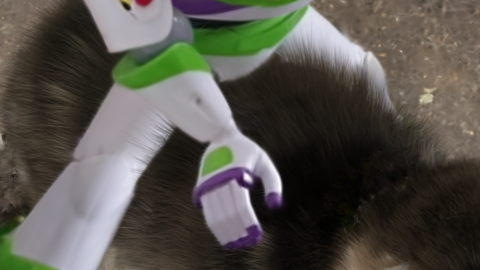
\includegraphics[width=0.49\linewidth]{images/composition/buzz_riding_cat/closeup_1.png}
 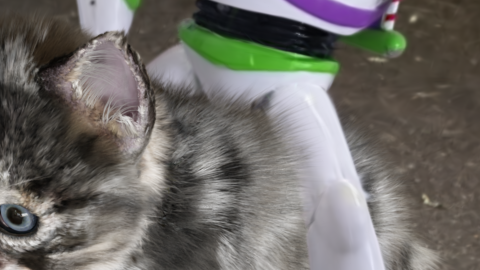
\includegraphics[width=0.49\linewidth]{images/composition/buzz_riding_cat/closeup_2.png}
 \caption*{(c) Fuzzy details rendered with Frosting - occlusions are correctly rendered}
  \end{subfigure}
  %
  \hfill
  %
  \begin{subfigure}{0.49\linewidth}
  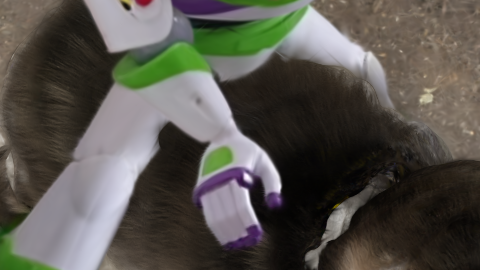
\includegraphics[width=0.49\linewidth]{images/composition/buzz_riding_cat/closeup_1_flat.png}
 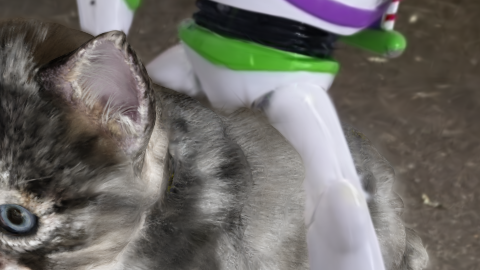
\includegraphics[width=0.49\linewidth]{images/composition/buzz_riding_cat/closeup_2_flat.png}
  \caption*{(d) Rendering with SuGaR~\cite{guedon2023sugar} - the fur does not occlude the legs correctly}
  \end{subfigure}
  %
  \caption{
  % original caption
  % \textbf{Complex scene composition with Frosting.} Frosting has editing capabilities similar to surface-based methods like SuGaR~\cite{guedon2023sugar}, but reaches better performance for rendering complex volumetric effects such as fuzzy materials. In this example, we were able to animate both Buzz and the kitten, changing their original pose (a) while preserving high-quality rendering (b): Contrary to SuGaR, very fine and fuzzy details such as the kitten's hair can be seen covering Buzz's legs in a realistic way (c).
  % final caption
  We propose to represent surfaces by a mesh covered with a ``Frosting'' layer of varying thickness and made of 3D Gaussians. This representation captures both complex volumetric effects created by fuzzy materials such as the cat's hair or grass as well as flat surfaces. 
  Built from RGB images only, it can be rendered in real-time and animated using traditional animation tools.
  In the example above, we were able to animate both Buzz and the kitten, changing their original pose (a) while preserving high-quality rendering (b): Contrary to SuGaR, very fine and fuzzy details such as the kitten's hair can be seen covering Buzz's legs in a realistic way (c).
  }
  \label{fig:sugar-comparison}
\end{figure}